\section{Remoção}

\begin{frame}[fragile]{Remoção em árvores binárias de busca}

    \begin{itemize}
	    \item A remoção em árvores binárias { depende da posição do nó} a ser removido

        \item São { três} casos:

        \begin{enumerate}
            \item o nó é uma folha, isto é, não tem filhos

            \item o nó tem um filho

            \item o nó tem dois filhos
        \end{enumerate}

        \item No primeiro caso, basta { remover} a referência do pai e {remover} o nó

        \item No segundo caso, a referência do { pai} é alterada para apontar para neto, e o nó é removido

        \item O terceiro caso não pode ser resolvido em um único passo

        \item Duas possíveis soluções são a remoção por fusão ou a remoção por cópia
    \end{itemize}
\end{frame} 

\begin{frame}[fragile]{Exemplo de remoção de nó sem filhos}

    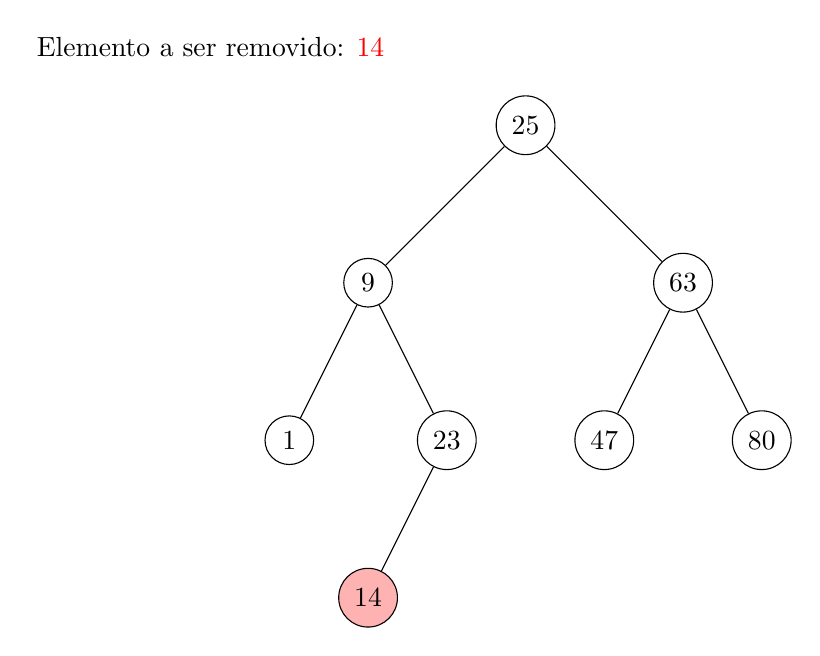
\begin{tikzpicture}

        \begin{scope}
            \node (X) at (1, 6) { Elemento a ser removido: \textcolor{red}{14}};

            \node[circle,draw] (D) at (5, 5) { $25$ };
            \node[circle,draw] (C) at (3, 3) { $9$ };
            \node[circle,draw] (E) at (7, 3) { $63$ };
            \node[circle,draw] (F) at (6, 1) { $47$ };
            \node[circle,draw] (A) at (2, 1) { $1$ };
            \node[circle,draw] (B) at (4, 1) { $23$ };
            \node[circle,draw] (G) at (8, 1) { $80$ };
            \node[circle,draw,fill=red!30] (H) at (3, -1) { $14$ };

            \draw (A) -- (C);
            \draw (B) -- (C);
            \draw (C) -- (D);
            \draw (D) -- (E);
            \draw (E) -- (F);
            \draw (E) -- (G);
            \draw (B) -- (H);

        \end{scope}
    \end{tikzpicture}

\end{frame}

\begin{frame}[fragile]{Exemplo de remoção de nó sem filhos}

    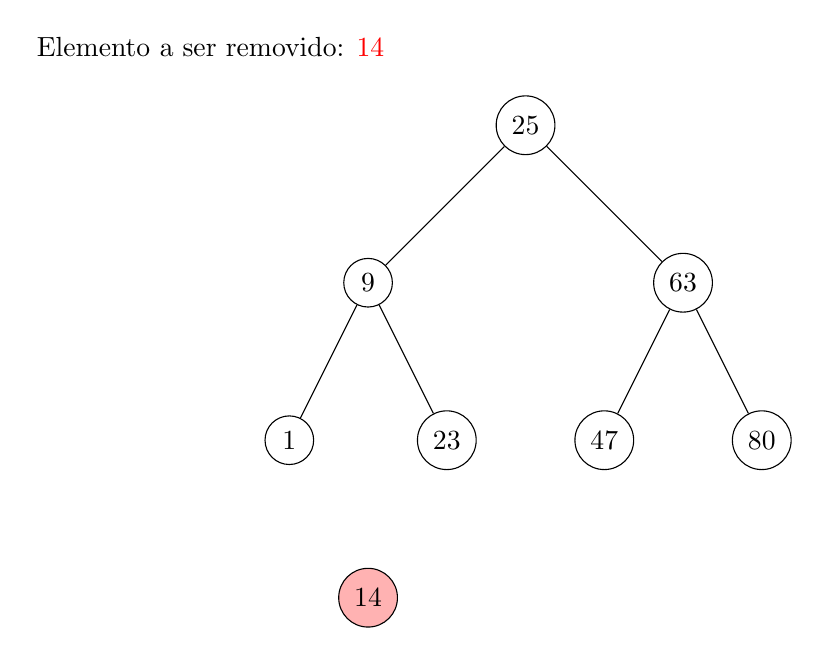
\begin{tikzpicture}

        \begin{scope}{shift={(3,1)}}
            \node (X) at (1, 6) { Elemento a ser removido: \textcolor{red}{14}};

            \node[circle,draw] (D) at (5, 5) { $25$ };
            \node[circle,draw] (C) at (3, 3) { $9$ };
            \node[circle,draw] (E) at (7, 3) { $63$ };
            \node[circle,draw] (F) at (6, 1) { $47$ };
            \node[circle,draw] (A) at (2, 1) { $1$ };
            \node[circle,draw] (B) at (4, 1) { $23$ };
            \node[circle,draw] (G) at (8, 1) { $80$ };
            \node[circle,draw,fill=red!30] (H) at (3, -1) { $14$ };

            \draw (A) -- (C);
            \draw (B) -- (C);
            \draw (C) -- (D);
            \draw (D) -- (E);
            \draw (E) -- (F);
            \draw (E) -- (G);

        \end{scope}
    \end{tikzpicture}

\end{frame}

\begin{frame}[fragile]{Exemplo de remoção de nó sem filhos}

    \begin{tikzpicture}

        \begin{scope}{shift={(3,1)}}
            \node (X) at (1, 6) { Elemento a ser removido: \textcolor{black}{14}};

            \node[circle,draw] (D) at (5, 5) { $25$ };
            \node[circle,draw] (C) at (3, 3) { $9$ };
            \node[circle,draw] (E) at (7, 3) { $63$ };
            \node[circle,draw] (F) at (6, 1) { $47$ };
            \node[circle,draw] (A) at (2, 1) { $1$ };
            \node[circle,draw] (B) at (4, 1) { $23$ };
            \node[circle,draw] (G) at (8, 1) { $80$ };
            \node[opacity=0,circle,draw,fill=red!30] (H) at (3, -1) { $14$ };

            \draw (A) -- (C);
            \draw (B) -- (C);
            \draw (C) -- (D);
            \draw (D) -- (E);
            \draw (E) -- (F);
            \draw (E) -- (G);

        \end{scope}
    \end{tikzpicture}

\end{frame}

\begin{frame}[fragile]{Exemplo de remoção de nó com apenas um filho}

    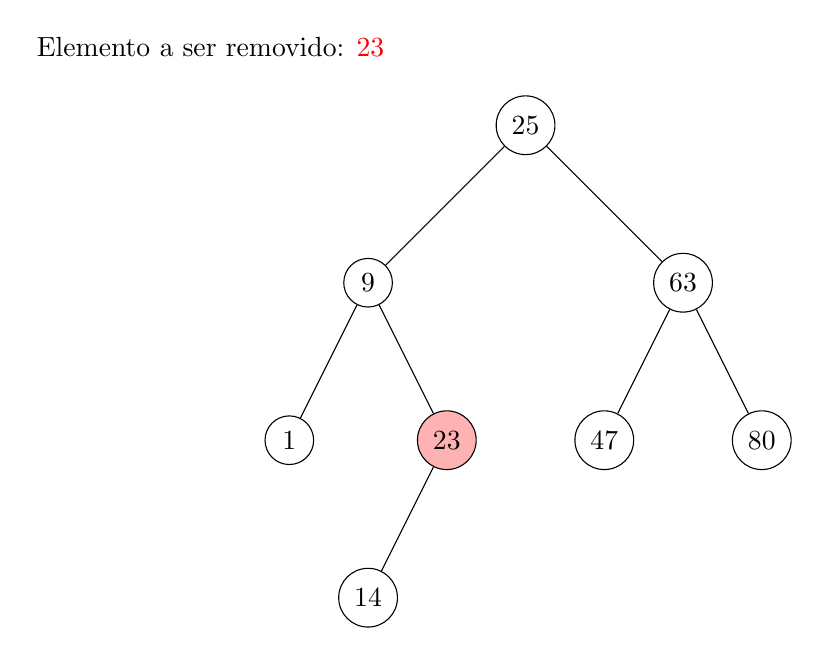
\begin{tikzpicture}

        \begin{scope}{shift={(3,1)}}
            \node (X) at (1, 6) { Elemento a ser removido: \textcolor{red}{23}};

            \node[circle,draw] (D) at (5, 5) { $25$ };
            \node[circle,draw] (C) at (3, 3) { $9$ };
            \node[circle,draw] (E) at (7, 3) { $63$ };
            \node[circle,draw] (F) at (6, 1) { $47$ };
            \node[circle,draw] (A) at (2, 1) { $1$ };
            \node[circle,draw,fill=red!30] (B) at (4, 1) { $23$ };
            \node[circle,draw] (G) at (8, 1) { $80$ };
            \node[circle,draw] (H) at (3, -1) { $14$ };

            \draw (A) -- (C);
            \draw (B) -- (C);
            \draw (C) -- (D);
            \draw (D) -- (E);
            \draw (E) -- (F);
            \draw (E) -- (G);
            \draw (B) -- (H);

        \end{scope}
    \end{tikzpicture}

\end{frame}

\begin{frame}[fragile]{Exemplo de remoção de nó com apenas um filho}

    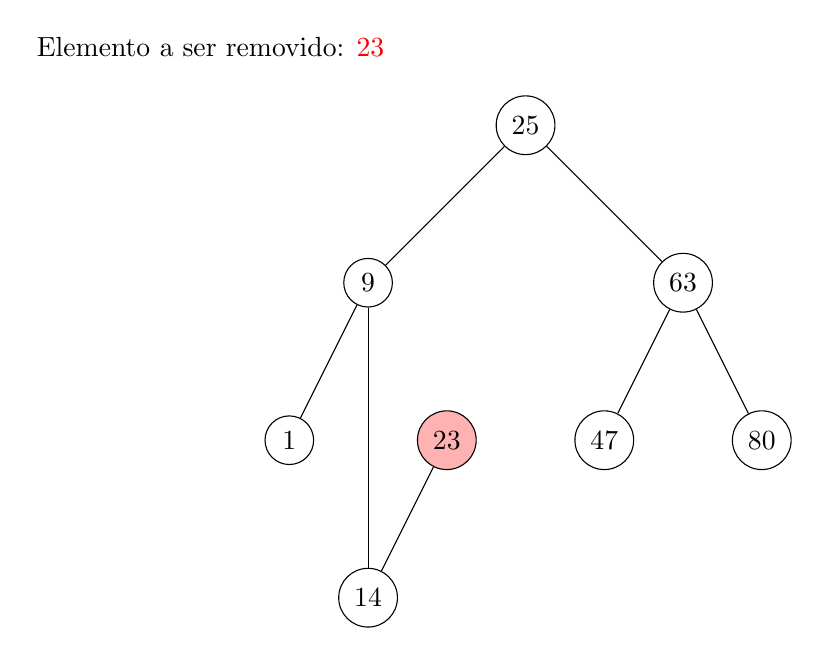
\begin{tikzpicture}

        \begin{scope}{shift={(3,1)}}
            \node (X) at (1, 6) { Elemento a ser removido: \textcolor{red}{23}};

            \node[circle,draw] (D) at (5, 5) { $25$ };
            \node[circle,draw] (C) at (3, 3) { $9$ };
            \node[circle,draw] (E) at (7, 3) { $63$ };
            \node[circle,draw] (F) at (6, 1) { $47$ };
            \node[circle,draw] (A) at (2, 1) { $1$ };
            \node[circle,draw,fill=red!30] (B) at (4, 1) { $23$ };
            \node[circle,draw] (G) at (8, 1) { $80$ };
            \node[circle,draw] (H) at (3, -1) { $14$ };

            \draw (A) -- (C);
            \draw (H) -- (C);
            \draw (C) -- (D);
            \draw (D) -- (E);
            \draw (E) -- (F);
            \draw (E) -- (G);
            \draw (B) -- (H);

        \end{scope}
    \end{tikzpicture}

\end{frame}

\begin{frame}[fragile]{Exemplo de remoção de nó com apenas um filho}

    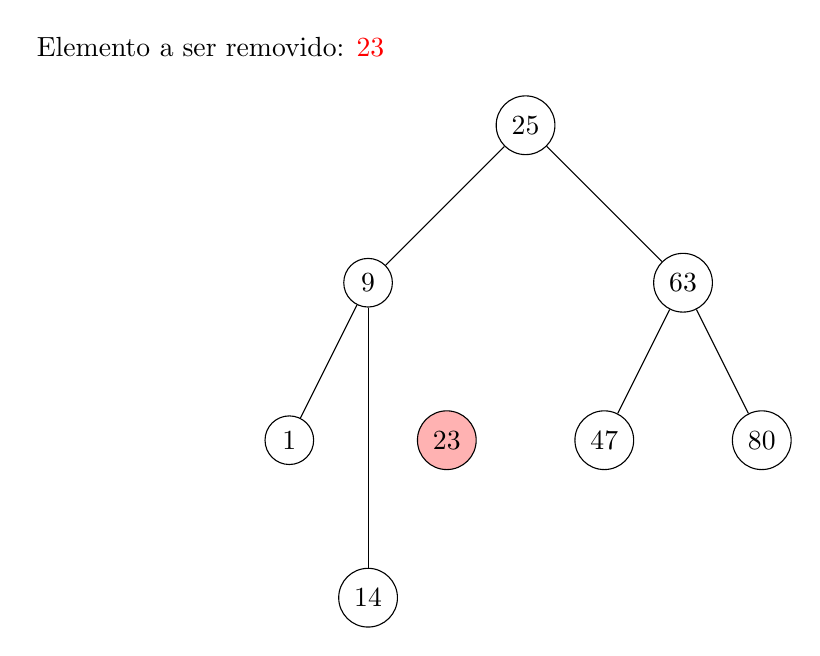
\begin{tikzpicture}

        \begin{scope}{shift={(3,1)}}
            \node (X) at (1, 6) { Elemento a ser removido: \textcolor{red}{23}};

            \node[circle,draw] (D) at (5, 5) { $25$ };
            \node[circle,draw] (C) at (3, 3) { $9$ };
            \node[circle,draw] (E) at (7, 3) { $63$ };
            \node[circle,draw] (F) at (6, 1) { $47$ };
            \node[circle,draw] (A) at (2, 1) { $1$ };
            \node[circle,draw,fill=red!30] (B) at (4, 1) { $23$ };
            \node[circle,draw] (G) at (8, 1) { $80$ };
            \node[circle,draw] (H) at (3, -1) { $14$ };

            \draw (A) -- (C);
            \draw (H) -- (C);
            \draw (C) -- (D);
            \draw (D) -- (E);
            \draw (E) -- (F);
            \draw (E) -- (G);
%            \draw (B) -- (H);

        \end{scope}
    \end{tikzpicture}

\end{frame}

\begin{frame}[fragile]{Exemplo de remoção de nó com apenas um filho}

    \begin{tikzpicture}

        \begin{scope}{shift={(3,1)}}
            \node (X) at (1, 6) { Elemento a ser removido: \textcolor{black}{23}};

            \node[circle,draw] (D) at (5, 5) { $25$ };
            \node[circle,draw] (C) at (3, 3) { $9$ };
            \node[circle,draw] (E) at (7, 3) { $63$ };
            \node[circle,draw] (F) at (6, 1) { $47$ };
            \node[circle,draw] (A) at (2, 1) { $1$ };
            \node[opacity=0,circle,draw,fill=red!30] (B) at (4, 1) { $23$ };
            \node[circle,draw] (G) at (8, 1) { $80$ };
            \node[circle,draw] (H) at (3, -1) { $14$ };

            \draw (A) -- (C);
            \draw (H) -- (C);
            \draw (C) -- (D);
            \draw (D) -- (E);
            \draw (E) -- (F);
            \draw (E) -- (G);
%            \draw (B) -- (H);

        \end{scope}
    \end{tikzpicture}

\end{frame}

\begin{frame}[fragile]\frametitle{Remoção por fusão}

	\begin{itemize}
		\item Esta técnica consiste em gerar uma nova árvore a partir das duas subárvores do nó a 
            ser removido

		\item Numa árvore binária de busca, qualquer elemento da subárvore à direita é maior do 
            que qualquer elemento da subárvore à esquerda

		\item Desta maneira, basta encontrar o nó mais à direita da subárvore à esquerda e 
            transformá-lo no pai da subárvore à direita

        \item São quatro passos para a remoção por fusão:

        \begin{enumerate}
            \item Localize o nó que deve ser removido (com dois filhos) e seu pai

            \item Na subárvore à esquerda, encontre o elemento mais à direita possível: 
                basta mover-se sempre para a direita até que se encontre um nó nulo

            \item Torne a raiz da subárvore à esquerda o novo filho do pai do nó a ser removido 

            \item Faça com que o nó mais à direita da subárvore à esquerda tenha como filho à 
                direita a subárvore à direita do nó a ser removido
        \end{enumerate}

        \item \textit{Corner case}: caso o nó seja a raiz, após a remoção a raiz deve apontar 
            para a raiz da subárvore à esquerda
    \end{itemize}

\end{frame}

\begin{frame}[fragile]{Exemplo de remoção por fusão}

    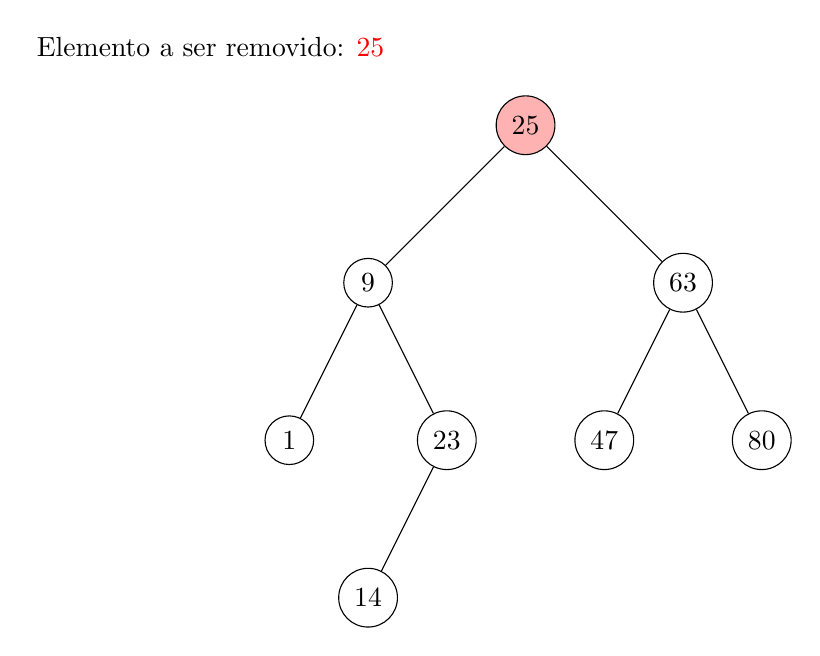
\begin{tikzpicture}

        \begin{scope}{shift={(3,1)}}
            \node (X) at (1, 6) { Elemento a ser removido: \textcolor{red}{25}};

            \node[circle,draw,fill=red!30] (D) at (5, 5) { $25$ };
            \node[circle,draw] (C) at (3, 3) { $9$ };
            \node[circle,draw] (E) at (7, 3) { $63$ };
            \node[circle,draw] (F) at (6, 1) { $47$ };
            \node[circle,draw] (A) at (2, 1) { $1$ };
            \node[circle,draw] (B) at (4, 1) { $23$ };
            \node[circle,draw] (G) at (8, 1) { $80$ };
            \node[circle,draw] (H) at (3, -1) { $14$ };

            \draw (A) -- (C);
            \draw (B) -- (C);
            \draw (C) -- (D);
            \draw (D) -- (E);
            \draw (E) -- (F);
            \draw (E) -- (G);
            \draw (B) -- (H);

        \end{scope}
    \end{tikzpicture}

\end{frame}

\begin{frame}[fragile]{Exemplo de remoção por fusão}

    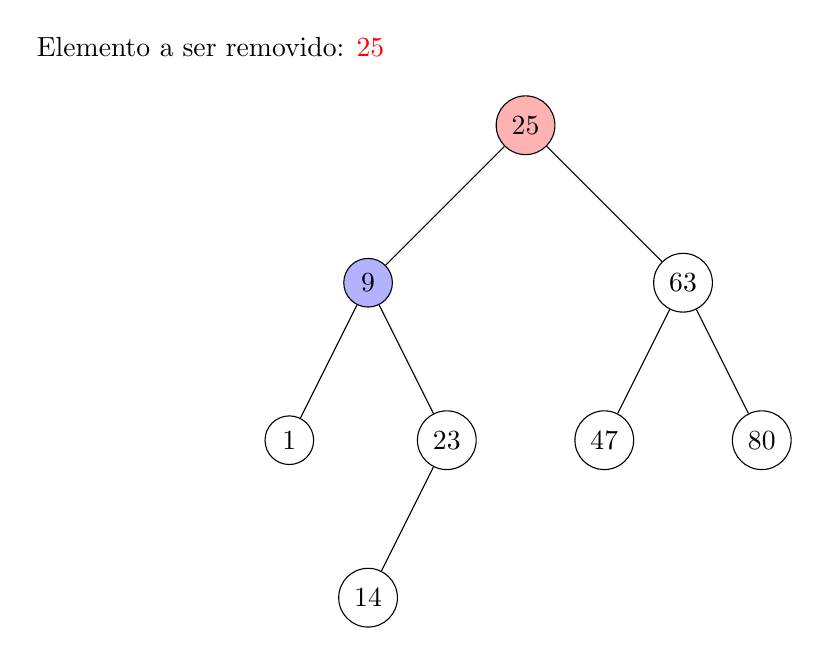
\begin{tikzpicture}

        \begin{scope}{shift={(3,1)}}
            \node (X) at (1, 6) { Elemento a ser removido: \textcolor{red}{25}};

            \node[circle,draw,fill=red!30] (D) at (5, 5) { $25$ };
            \node[circle,draw,fill=blue!30] (C) at (3, 3) { $9$ };
            \node[circle,draw] (E) at (7, 3) { $63$ };
            \node[circle,draw] (F) at (6, 1) { $47$ };
            \node[circle,draw] (A) at (2, 1) { $1$ };
            \node[circle,draw] (B) at (4, 1) { $23$ };
            \node[circle,draw] (G) at (8, 1) { $80$ };
            \node[circle,draw] (H) at (3, -1) { $14$ };

            \draw (A) -- (C);
            \draw (B) -- (C);
            \draw (C) -- (D);
            \draw (D) -- (E);
            \draw (E) -- (F);
            \draw (E) -- (G);
            \draw (B) -- (H);

        \end{scope}
    \end{tikzpicture}

\end{frame}

\begin{frame}[fragile]{Exemplo de remoção por fusão}

    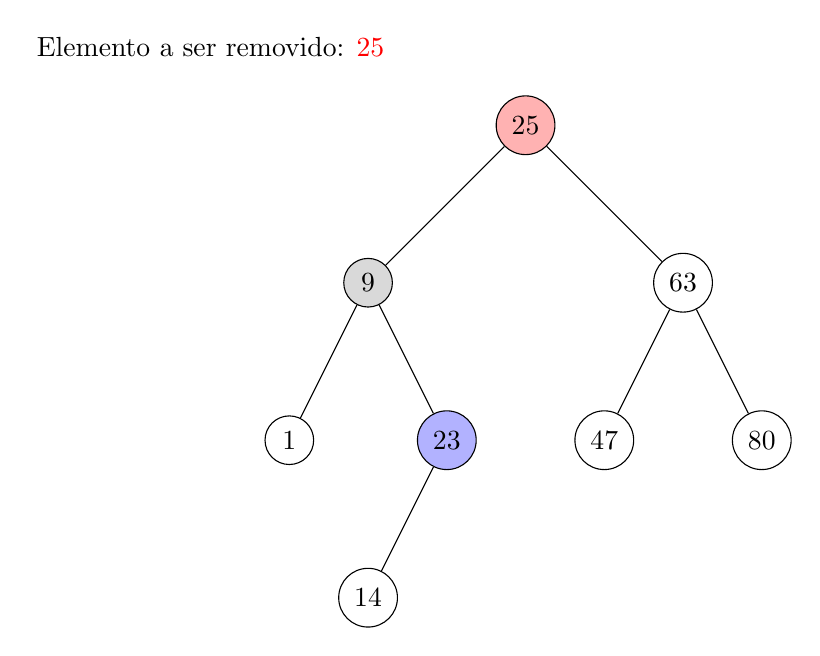
\begin{tikzpicture}

        \begin{scope}{shift={(3,1)}}
            \node (X) at (1, 6) { Elemento a ser removido: \textcolor{red}{25}};

            \node[circle,draw,fill=red!30] (D) at (5, 5) { $25$ };
            \node[circle,draw,fill=gray!30] (C) at (3, 3) { $9$ };
            \node[circle,draw] (E) at (7, 3) { $63$ };
            \node[circle,draw] (F) at (6, 1) { $47$ };
            \node[circle,draw] (A) at (2, 1) { $1$ };
            \node[circle,draw,fill=blue!30] (B) at (4, 1) { $23$ };
            \node[circle,draw] (G) at (8, 1) { $80$ };
            \node[circle,draw] (H) at (3, -1) { $14$ };

            \draw (A) -- (C);
            \draw (B) -- (C);
            \draw (C) -- (D);
            \draw (D) -- (E);
            \draw (E) -- (F);
            \draw (E) -- (G);
            \draw (B) -- (H);

        \end{scope}
    \end{tikzpicture}

\end{frame}

\begin{frame}[fragile]{Exemplo de remoção por fusão}

    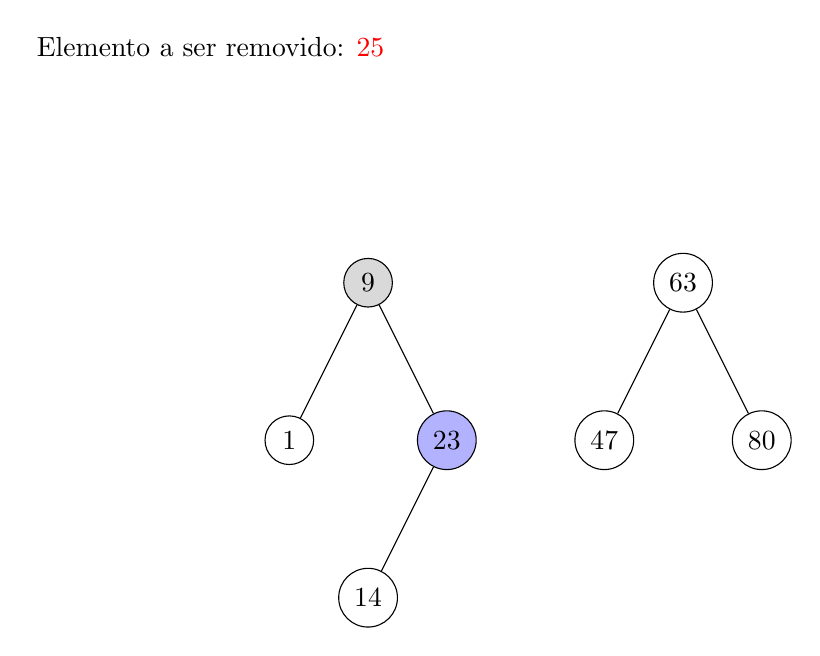
\begin{tikzpicture}

        \begin{scope}{shift={(3,1)}}
            \node (X) at (1, 6) { Elemento a ser removido: \textcolor{red}{25}};

            \node[opacity=0,circle,draw,fill=red!30] (D) at (5, 5) { $25$ };
            \node[circle,draw,fill=gray!30] (C) at (3, 3) { $9$ };
            \node[circle,draw] (E) at (7, 3) { $63$ };
            \node[circle,draw] (F) at (6, 1) { $47$ };
            \node[circle,draw] (A) at (2, 1) { $1$ };
            \node[circle,draw,fill=blue!30] (B) at (4, 1) { $23$ };
            \node[circle,draw] (G) at (8, 1) { $80$ };
            \node[circle,draw] (H) at (3, -1) { $14$ };

            \draw (A) -- (C);
            \draw (B) -- (C);
            \draw (E) -- (F);
            \draw (E) -- (G);
            \draw (B) -- (H);

        \end{scope}
    \end{tikzpicture}

\end{frame}

\begin{frame}[fragile]{Exemplo de remoção por fusão}

    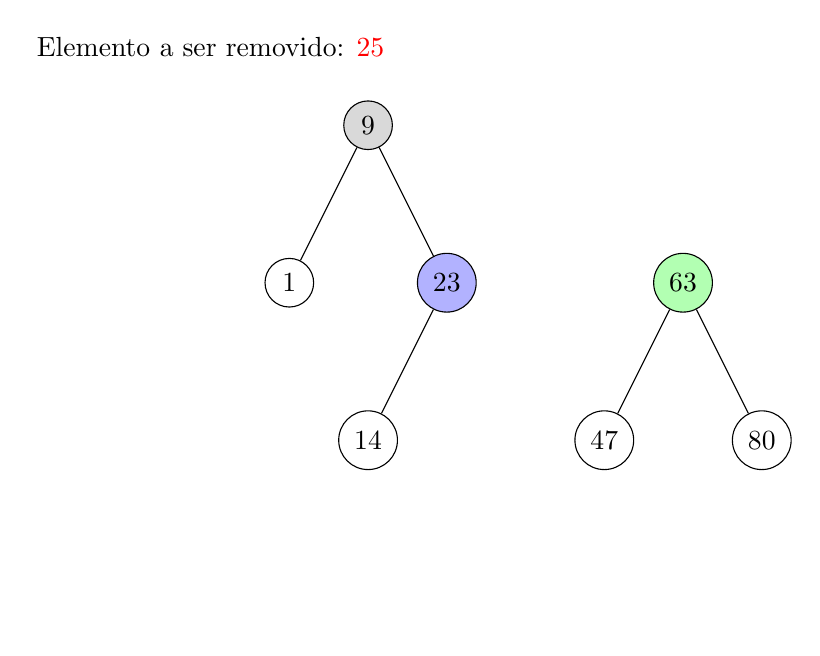
\begin{tikzpicture}

        \begin{scope}{shift={(3,1)}}
            \node (X) at (1, 6) { Elemento a ser removido: \textcolor{red}{25}};

            \node[opacity=0,circle,draw,fill=red!30] (D) at (5, 5) { $25$ };
            \node[circle,draw,fill=gray!30] (C) at (3, 5) { $9$ };
            \node[circle,draw,fill=green!30] (E) at (7, 3) { $63$ };
            \node[circle,draw] (F) at (6, 1) { $47$ };
            \node[circle,draw] (A) at (2, 3) { $1$ };
            \node[circle,draw,fill=blue!30] (B) at (4, 3) { $23$ };
            \node[circle,draw] (G) at (8, 1) { $80$ };
            \node[circle,draw] (H) at (3, 1) { $14$ };
            \node[opacity=0,circle,draw] (I) at (3, -1) { $14$ };

            \draw (A) -- (C);
            \draw (B) -- (C);
            \draw (E) -- (F);
            \draw (E) -- (G);
            \draw (B) -- (H);

        \end{scope}
    \end{tikzpicture}

\end{frame}

\begin{frame}[fragile]{Exemplo de remoção por fusão}

    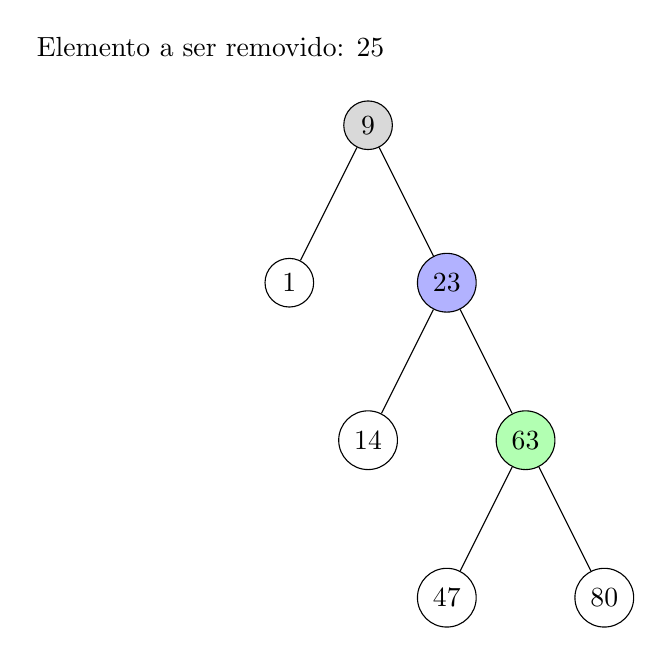
\begin{tikzpicture}

        \begin{scope}{shift={(3,1)}}
            \node (X) at (1, 6) { Elemento a ser removido: \textcolor{black}{25}};

            \node[opacity=0,circle,draw,fill=red!30] (D) at (5, 5) { $25$ };
            \node[circle,draw,fill=gray!30] (C) at (3, 5) { $9$ };
            \node[circle,draw,fill=green!30] (E) at (5, 1) { $63$ };
            \node[circle,draw] (F) at (4, -1) { $47$ };
            \node[circle,draw] (A) at (2, 3) { $1$ };
            \node[circle,draw,fill=blue!30] (B) at (4, 3) { $23$ };
            \node[circle,draw] (G) at (6, -1) { $80$ };
            \node[circle,draw] (H) at (3, 1) { $14$ };
            \node[opacity=0,circle,draw] (I) at (3, -1) { $14$ };

            \draw (A) -- (C);
            \draw (B) -- (C);
            \draw (B) -- (E);
            \draw (E) -- (F);
            \draw (E) -- (G);
            \draw (B) -- (H);

        \end{scope}
    \end{tikzpicture}

\end{frame}


\begin{frame}[fragile]{Implementação da remoção por fusão}
    \inputsnippet{cpp}{1}{20}{codes/delete_by_merging.cpp}
\end{frame}

\begin{frame}[fragile]{Implementação da remoção por fusão}
    \inputsnippet{cpp}{21}{36}{codes/delete_by_merging.cpp}
\end{frame}

\begin{frame}[fragile]{Implementação da remoção por fusão}
    \inputsnippet{cpp}{37}{57}{codes/delete_by_merging.cpp}
\end{frame}

\begin{frame}[fragile]{Remoção por cópia}

	\begin{itemize}
		\item Algoritmo proposto por Donald Knuth e Thomas Hibbard

		\item Ele reduz o caso de um nó ter dois filhos para um dos casos anteriores: ou 
            o nó não tem filhos ou tem apenas um

		\item Isto é feito substituíndo a informação do nó a ser deletado pela informação do nó 
                mais à direita da subárvore à esquerda, apagando este nó em seguida

        \item Os quatro passos da remoção por cópia são:
        \begin{enumerate}
            \item Localize o nó com dois filhos que deve ser removido

            \item Na subárvore à esquerda, encontre o elemento mais à direita possível

            \item Substitua a informação do nó a ser removido pela informação do nó localizado 
                no passo anterior

            \item Remova o nó localizado no segundo passo
        \end{enumerate}
    \end{itemize}
\end{frame}  

\begin{frame}[fragile]{Exemplo de remoção por cópia}

    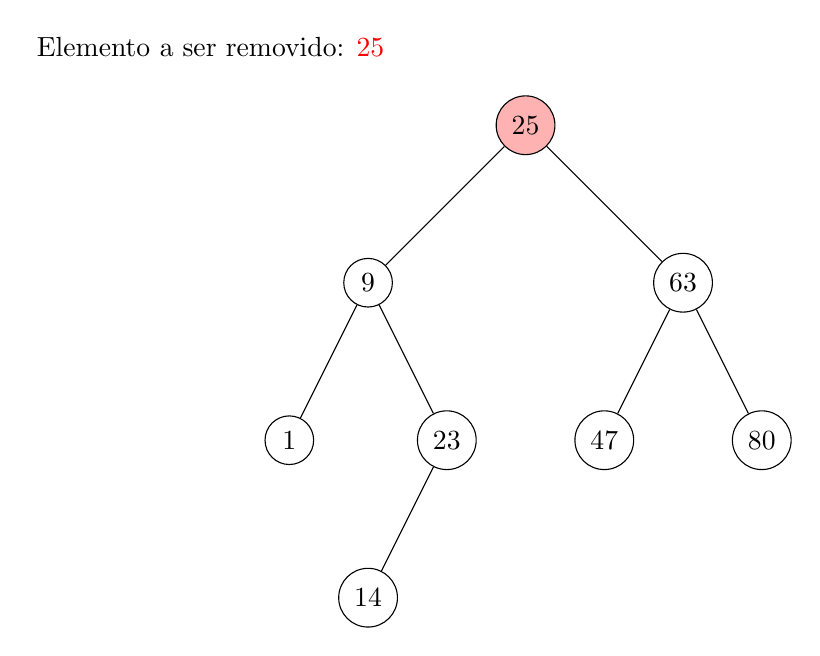
\begin{tikzpicture}

        \begin{scope}{shift={(3,1)}}
            \node (X) at (1, 6) { Elemento a ser removido: \textcolor{red}{25}};

            \node[circle,draw,fill=red!30] (D) at (5, 5) { $25$ };
            \node[circle,draw] (C) at (3, 3) { $9$ };
            \node[circle,draw] (E) at (7, 3) { $63$ };
            \node[circle,draw] (F) at (6, 1) { $47$ };
            \node[circle,draw] (A) at (2, 1) { $1$ };
            \node[circle,draw] (B) at (4, 1) { $23$ };
            \node[circle,draw] (G) at (8, 1) { $80$ };
            \node[circle,draw] (H) at (3, -1) { $14$ };

            \draw (A) -- (C);
            \draw (B) -- (C);
            \draw (C) -- (D);
            \draw (D) -- (E);
            \draw (E) -- (F);
            \draw (E) -- (G);
            \draw (B) -- (H);

        \end{scope}
    \end{tikzpicture}

\end{frame}

\begin{frame}[fragile]{Exemplo de remoção por cópia}

    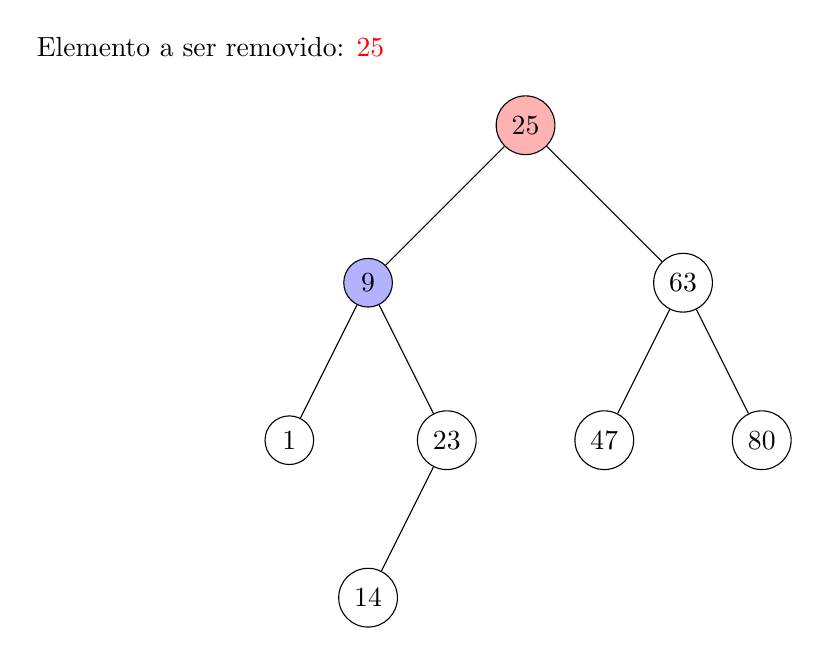
\begin{tikzpicture}

        \begin{scope}{shift={(3,1)}}
            \node (X) at (1, 6) { Elemento a ser removido: \textcolor{red}{25}};

            \node[circle,draw,fill=red!30] (D) at (5, 5) { $25$ };
            \node[circle,draw,fill=blue!30] (C) at (3, 3) { $9$ };
            \node[circle,draw] (E) at (7, 3) { $63$ };
            \node[circle,draw] (F) at (6, 1) { $47$ };
            \node[circle,draw] (A) at (2, 1) { $1$ };
            \node[circle,draw] (B) at (4, 1) { $23$ };
            \node[circle,draw] (G) at (8, 1) { $80$ };
            \node[circle,draw] (H) at (3, -1) { $14$ };

            \draw (A) -- (C);
            \draw (B) -- (C);
            \draw (C) -- (D);
            \draw (D) -- (E);
            \draw (E) -- (F);
            \draw (E) -- (G);
            \draw (B) -- (H);

        \end{scope}
    \end{tikzpicture}

\end{frame}

\begin{frame}[fragile]{Exemplo de remoção por cópia}

    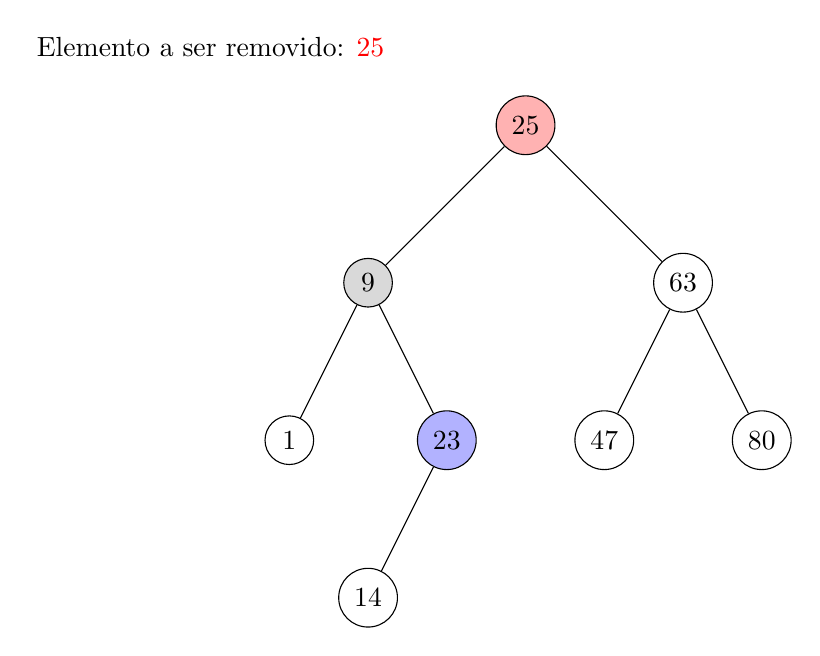
\begin{tikzpicture}

        \begin{scope}{shift={(3,1)}}
            \node (X) at (1, 6) { Elemento a ser removido: \textcolor{red}{25}};

            \node[circle,draw,fill=red!30] (D) at (5, 5) { $25$ };
            \node[circle,draw,fill=gray!30] (C) at (3, 3) { $9$ };
            \node[circle,draw] (E) at (7, 3) { $63$ };
            \node[circle,draw] (F) at (6, 1) { $47$ };
            \node[circle,draw] (A) at (2, 1) { $1$ };
            \node[circle,draw,fill=blue!30] (B) at (4, 1) { $23$ };
            \node[circle,draw] (G) at (8, 1) { $80$ };
            \node[circle,draw] (H) at (3, -1) { $14$ };

            \draw (A) -- (C);
            \draw (B) -- (C);
            \draw (C) -- (D);
            \draw (D) -- (E);
            \draw (E) -- (F);
            \draw (E) -- (G);
            \draw (B) -- (H);

        \end{scope}
    \end{tikzpicture}

\end{frame}

\begin{frame}[fragile]{Exemplo de remoção por cópia}

    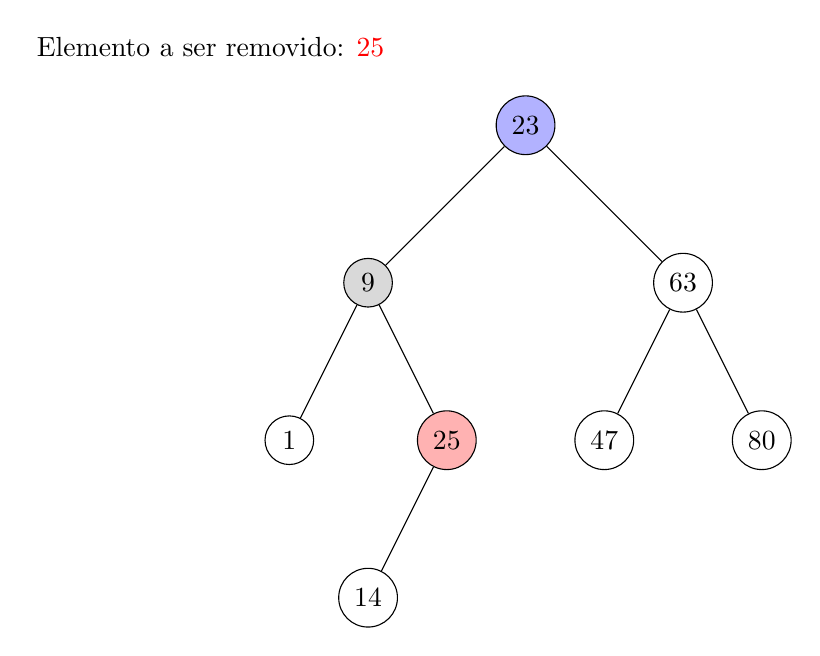
\begin{tikzpicture}

        \begin{scope}{shift={(3,1)}}
            \node (X) at (1, 6) { Elemento a ser removido: \textcolor{red}{25}};

            \node[circle,draw,fill=blue!30] (D) at (5, 5) { $23$ };
            \node[circle,draw,fill=gray!30] (C) at (3, 3) { $9$ };
            \node[circle,draw] (E) at (7, 3) { $63$ };
            \node[circle,draw] (F) at (6, 1) { $47$ };
            \node[circle,draw] (A) at (2, 1) { $1$ };
            \node[circle,draw,fill=red!30] (B) at (4, 1) { $25$ };
            \node[circle,draw] (G) at (8, 1) { $80$ };
            \node[circle,draw] (H) at (3, -1) { $14$ };

            \draw (A) -- (C);
            \draw (B) -- (C);
            \draw (C) -- (D);
            \draw (D) -- (E);
            \draw (E) -- (F);
            \draw (E) -- (G);
            \draw (B) -- (H);

        \end{scope}
    \end{tikzpicture}

\end{frame}

\begin{frame}[fragile]{Exemplo de remoção por cópia}

    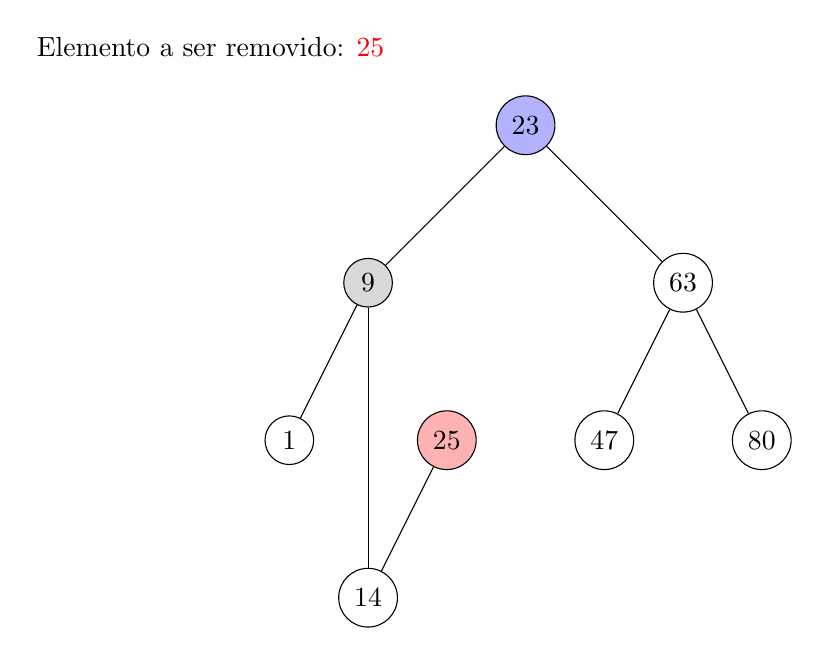
\begin{tikzpicture}

        \begin{scope}{shift={(3,1)}}
            \node (X) at (1, 6) { Elemento a ser removido: \textcolor{red}{25}};

            \node[circle,draw,fill=blue!30] (D) at (5, 5) { $23$ };
            \node[circle,draw,fill=gray!30] (C) at (3, 3) { $9$ };
            \node[circle,draw] (E) at (7, 3) { $63$ };
            \node[circle,draw] (F) at (6, 1) { $47$ };
            \node[circle,draw] (A) at (2, 1) { $1$ };
            \node[circle,draw,fill=red!30] (B) at (4, 1) { $25$ };
            \node[circle,draw] (G) at (8, 1) { $80$ };
            \node[circle,draw] (H) at (3, -1) { $14$ };

            \draw (A) -- (C);
            \draw (H) -- (C);
            \draw (C) -- (D);
            \draw (D) -- (E);
            \draw (E) -- (F);
            \draw (E) -- (G);
            \draw (B) -- (H);

        \end{scope}
    \end{tikzpicture}

\end{frame}

\begin{frame}[fragile]{Exemplo de remoção por cópia}

    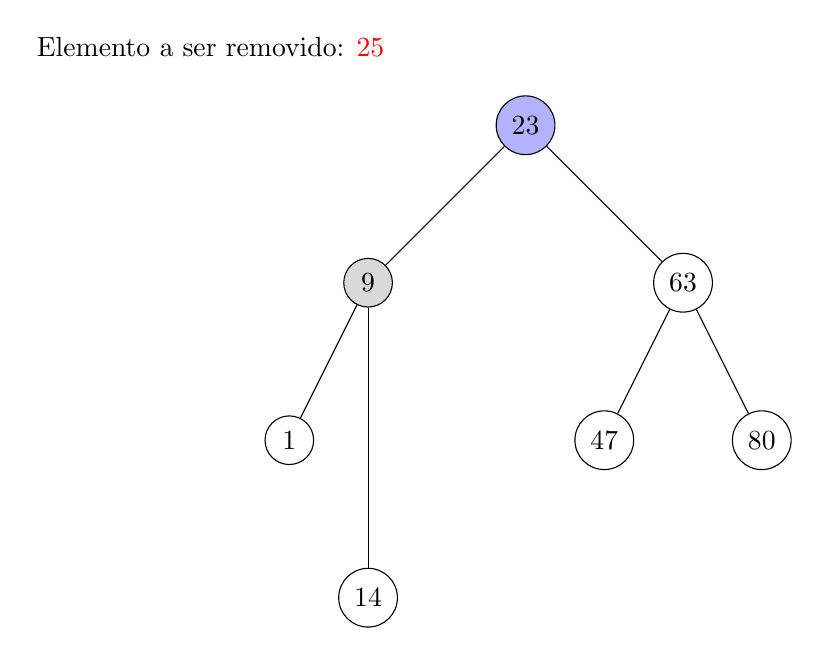
\begin{tikzpicture}

        \begin{scope}{shift={(3,1)}}
            \node (X) at (1, 6) { Elemento a ser removido: \textcolor{red}{25}};

            \node[circle,draw,fill=blue!30] (D) at (5, 5) { $23$ };
            \node[circle,draw,fill=gray!30] (C) at (3, 3) { $9$ };
            \node[circle,draw] (E) at (7, 3) { $63$ };
            \node[circle,draw] (F) at (6, 1) { $47$ };
            \node[circle,draw] (A) at (2, 1) { $1$ };
            \node[circle,draw] (G) at (8, 1) { $80$ };
            \node[circle,draw] (H) at (3, -1) { $14$ };

            \draw (A) -- (C);
            \draw (H) -- (C);
            \draw (C) -- (D);
            \draw (D) -- (E);
            \draw (E) -- (F);
            \draw (E) -- (G);
%            \draw (B) -- (H);

        \end{scope}
    \end{tikzpicture}

\end{frame}

\begin{frame}[fragile]{Implementação da remoção por cópia}
    \inputsnippet{cpp}{1}{20}{codes/delete_by_copying.cpp}
\end{frame}

\begin{frame}[fragile]{Implementação da remoção por cópia}
    \inputsnippet{cpp}{21}{36}{codes/delete_by_copying.cpp}
\end{frame}

\begin{frame}[fragile]{Implementação da remoção por cópia}
    \inputsnippet{cpp}{37}{57}{codes/delete_by_copying.cpp}
\end{frame}

\begin{frame}[fragile]{Notas sobre os algoritmos de remoção}

    \begin{itemize}
        \item De forma semelhante à inserção, ambos algoritmos de remoção tem complexidade 
            $O(N)$ no pior caso (folha de uma árvore degenerada com $N$ nós)

        \item Observe que a remoção por fusão aumenta ou mantém a altura da árvore

        \item Já a remoção por cópia mantém ou diminui a altura da árvore

        \item Efetivamente, a complexidade de ambos algoritmos é $O(h)$, onde $h$ é a altura da
            árvore

        \item Em uma árvore balanceada, $h = O(\log N)$, o que melhora a complexidade de 
            ambos algoritmos

        \item Para manter uma árvore balanceada, a remoção por cópia é mais adequada do que
            a remoção por fusão

        \item Contudo, como já dito, a inserção pode desbalancear a árvore

        \item Logo é preciso alterar a inserção para que o balanceamento seja preservado
    \end{itemize}

\end{frame}
